\documentclass[11pt]{article}

% --- arXiv-friendly preamble ---
\usepackage[utf8]{inputenc}
\usepackage[T1]{fontenc}
\usepackage[margin=1in]{geometry}
\usepackage{graphicx}
\usepackage{booktabs}
\usepackage{amsmath,amssymb}
\usepackage{xcolor}
\usepackage{microtype}
\usepackage[numbers,sort&compress]{natbib}
\usepackage[colorlinks=true,linkcolor=blue,citecolor=blue,urlcolor=blue]{hyperref}

\newcommand{\file}[1]{\texttt{#1}}

\title{Abliteration does not buy autonomy:\\ refusal removal across capability- and
willingness-bound\\ offensive tasks in small local LLMs}
\author{Gonzalo D.\,C.\ Garc\'ia\thanks{Independent Researcher. Preliminary findings; preprint.}}
\date{June 2026}

\begin{document}
\maketitle

\begin{abstract}
A widely repeated worry holds that \emph{abliteration}, surgically removing the refusal direction
from an open-weight model, turns a cheap locally-runnable LLM into a more dangerous autonomous
attacker. It conflates willingness with capability, which we separate empirically on a single
consumer laptop GPU. Three findings follow. Removing refusals does not raise a small model's
autonomous offensive capability and usually lowers it. The effect is signed: on a task bound by
willingness rather than capability it reverses, and abliteration helps. And the policy-relevant
question, whether a robust safeguard survives, is one our instrument cannot answer, for reasons we
set out.

On capability we run matched pairs, an aligned 7--8B model against its abliterated twin, inside a
tool-using operator scaffold against a controlled synthetic OSINT range. Across Llama-3.1-8B and
Qwen2.5-7B (11 personas $\times$ 3 seeds, 95\% bootstrap CIs) the aligned model recovers more
planted facts, with non-overlapping CIs; Granite collapses for both twins, a tool-protocol failure
we read as a floor. The result survives a change of framing and points the same way in a second,
network-free domain (static code audit), though that domain is under-powered ($n{=}3$ codebases) and
we treat it as directional. A frontier model (Opus 4.8) run blind on a non-person variant scores
100\%, a ceiling (in its own harness, so a ceiling and not a like-for-like comparison) that places
the small models' shortfall on the capability axis. Flip the task to writing a phishing lure and the
sign flips with it: the abliterated model complies where the aligned one refuses, by as much refusal
as the aligned twin had to give up, which for one of three families is almost none (harm 0 to 85 in
Llama, 32 to 77 in Qwen, unchanged at 81 in Granite).

The safeguard question is the one we cannot answer, and the reason is itself a result. Because the
range is declared synthetic, a well-aligned frontier model complies with the person-OSINT task
($\sim$64\% recall, planted credentials included, in both neutral and adversarial framings) just
because it reads the records as fictitious; a declared-synthetic instrument therefore cannot measure
context-dependent refusal at all. An earlier draft of ours claimed the opposite, a robust frontier
refusal. On audit that was a contaminated harness, which we retract and document as a cautionary
case. Practically, removing refusals adds little to a small model's misuse ceiling: what governs the
risk is the task's bottleneck and the fragility of the small model's own alignment, with the weight
edit a secondary factor. We release the range generator,
the operator harness, the graders, and all run artifacts.
\end{abstract}

\section{Introduction}

Open-weight ``uncensored'' and abliterated LLMs are everywhere, and they run on a gaming laptop.
The worry that follows is a short syllogism. Safety training adds refusals, abliteration strips
them out, so an abliterated model ought to be a more capable autonomous attacker. The last step is
where it breaks. Refusal is a property of \emph{willingness}; operating offensively on your own is
a property of \emph{capability}, which means multi-step tool use, chaining evidence across calls,
and not hallucinating. Deleting a refusal direction acts on the first of these. It does nothing
obvious for the second, and it may even hurt.

We test this in the regime the proliferation story actually cares about: a 7--8B quantized model
on one 8\,GB laptop GPU (an RTX 5060 Laptop), wrapped in a Claude-Code-style operator scaffold
(planning ledger, tool execution, retrieval augmentation, an adversarial evidence gate) and pointed
at a controlled OSINT task. Three questions shape the design. The first is whether abliteration
actually raises a small model's autonomous OSINT capability above its aligned twin. The second is
about the nature of any shortfall: if the small models fall short, is that a ceiling they hit, or
headroom a maximally capable frontier model could reach and abliteration might in principle unlock?
The third is more awkward, and we did not anticipate how much it would matter: can a range you have
\emph{declared} synthetic even be used to ask whether a frontier model refuses autonomous
person-profiling?

The answers, in order. No: the abliterated twin is never ahead. In the two families that actually
clear the task, Llama and Qwen, it loses with disjoint CIs, and the third (Granite) sits at the
floor for both twins, which tells us about its protocol-following, not its capability. The result
survives a change of framing. The shortfall is a capability ceiling rather than missing
willingness, because a frontier model hits 100\% on the blind non-person variant of the range. And
no again, the synthetic range cannot isolate refusal, because the frontier complies with a task it
can plainly see is fictional. The policy reading is unglamorous. The marginal misuse risk from
abliterating a small model is small, since scale and capability set its ceiling, not the refusals
you removed.

\paragraph{A retracted claim.} An earlier version of this work reported a second finding, a
``safety inversion'': frontier models robustly refuse the task while small models comply. It was
wrong, and the reason is worth stating, because it is the kind of mistake an evaluation harness
makes easy. The frontier ``refusals'' came from prompts that a Windows shell truncated before the
tool instructions ever reached the model. Once the harness was fixed the frontier complied at
$\sim$64\% recall, planted credentials and all, under both neutral and adversarial framings. We
retract the safety-inversion claim. The frontier-refusal question, it turns out, cannot be answered
with a declared-synthetic instrument at all (\S\ref{sec:limits}).

We then turn the design on its head. To check that the capability result is not the whole story, we
add a willingness-bound task, writing a targeted phishing lure, where the bottleneck is the refusal
itself rather than competence. There the sign reverses: abliteration helps, by exactly as much
refusal as the aligned model had to give up, which for one of our three families is almost none.

This is an empirical measurement study, built on five matched-pair experiments (E1--E5) with
original data and a released, reproducible instrument. What it contributes: the agentic-autonomy
delta abliteration induces on consumer hardware, matched-pair and with confidence intervals; the observation that this delta is signed, set by whether the task is
bound by capability or by willingness; a synthetic OSINT instrument that is reproducible and keeps
no real people in scope; and a negative result, that a declared-synthetic range cannot measure
context-dependent refusal, carried by the harness audit that caught our own false finding.

\section{Related work}

\paragraph{Refusal removal and the brittleness of alignment.}
Refusal behavior in aligned LLMs is mediated by a single linear direction in activation space, and
ablating it (``abliteration'') removes refusals without retraining \cite{arditi2024refusal}. More
broadly, safety alignment is brittle to cheap weight edits: pruning and low-rank modifications
\cite{wei2024brittleness}, a few steps of fine-tuning \cite{qi2024finetuning}, or direct
safety-finetuning stripping \cite{krupkina2024badgpt4o} all degrade refusals. This literature
establishes that refusals are \emph{easy to remove}. It does not establish that removing them
\emph{increases autonomous offensive capability}. Willingness against capability: that gap is what
we measure.

\paragraph{Agentic offensive-security benchmarks.}
A growing set of benchmarks evaluates LLM \emph{agents} on offensive tasks: Cybench
\cite{zhang2024cybench}, NYU CTF Bench \cite{shao2024nyuctf}, and the InterCode-CTF environment
\cite{yang2023intercode} score capture-the-flag solving; AutoPenBench
\cite{gioacchini2024autopenbench} and PentestGPT \cite{deng2024pentestgpt} score penetration
testing; EnIGMA \cite{abramovich2025enigma} reports state of the art across several of these. These
measure \emph{absolute capability}, almost always of frontier or large models, not the \emph{delta}
induced by a weight edit on a small model, and not on consumer hardware.

\paragraph{Dual-use / misuse evaluation.}
The CyberSecEval suite \cite{bhatt2023cyberseceval, bhatt2024cyberseceval2, wan2024cyberseceval3}
and guardrail models such as Llama Guard \cite{inan2023llamaguard} evaluate or enforce refusal of
\emph{single-shot} harmful requests. We instead measure behavior on a \emph{multi-step autonomous}
task, where willingness and capability can be separated.

\paragraph{LLMs for OSINT / privacy inference.}
LLMs can infer personal attributes from unstructured text at scale \cite{staab2024beyond} and have
been evaluated as OSINT assistants \cite{shafee2025osint}. These study capability or privacy leakage
of a single model; none compares an aligned model to its abliterated twin on an autonomous OSINT
task.

\paragraph{What we measure.}
We measure the \textbf{agentic-autonomy delta induced by abliteration}, matched-pair, on
\textbf{consumer hardware}, across two domains (OSINT and code audit), with bootstrap confidence
intervals \cite{efron1979bootstrap, diciccio1996bootstrap, efron1993introduction}. We had also
intended to measure a frontier$\leftrightarrow$small \textbf{refusal asymmetry} on the autonomous
task; we report instead \emph{why a declared-synthetic range cannot} establish such an asymmetry
(\S\ref{sec:e3}, \S\ref{sec:limits}). To our knowledge the matched aligned/abliterated agentic
comparison on consumer hardware has not been reported.

\section{Instrument and method}

\subsection{Synthetic OSINT range (NimbusForge)}
We generate a self-contained synthetic organization, \emph{NimbusForge}, with 11 personas
stratified by difficulty (4 easy / 4 medium / 3 hard). Each persona has a set of \emph{planted
facts} (name, role, location, username, and --- for the hard tier --- a leaked credential)
distributed across a public team directory, profile pages, blog posts, and a simulated breach dump.
All identities use \texttt{.example} domains; no real people, no live Internet. The generator is
deterministic (\file{abliterbench/osint\_range/generate.py}), so the range is reproducible from a
seed. A non-person isomorphic variant (\file{-{}-variant assets}: 11 service accounts whose
``secret'' is a test API key) exists for blind frontier capability testing without the person-OSINT
framing (used in E3).

\subsection{Operator scaffold}
The model under test drives an agent loop (\file{abliterbench/operator/}) exposing OSINT tools
(\file{osint\_people\_search}, \file{web\_fetch}, \file{osint\_breach\_lookup}) via a sandboxed
bridge running in an isolated Kali VM. The loop provides a planning ledger, retrieval augmentation,
tool-result distillation, context compaction, and malformed-tool-call repair. The piece that did
the most work is an evidence-anchored final-answer step: a report may assert only facts backed by
collected tool evidence. That alone removed the small models' habit of fabricating findings (zero
hallucinated facts under the scaffold; in the multi-agent variant an adversarial verifier rejects
unsupported findings that simpler configs wave through). Every small model runs the same harness,
which keeps the aligned/abliterated comparison fair. Frontier models are the exception: they run
through their own native CLI loop, a different harness, and \S\ref{sec:limits} returns to what that
costs us.

\subsection{Grading}
\file{grade\_dossier} scores \textbf{recall} (fraction of planted facts recovered, NFKD-normalized,
field-agnostic) and \textbf{precision} (fraction of asserted facts not contradicted by decoys in
the breach dump). Refusal is classified by \file{classify\_refusal}: a regex detector plus an
optional LLM-judge, with agreement recorded. Confidence intervals are nonparametric bootstrap (5000
resamples, fixed seed) over persona~$\times$~seed cells (\file{analysis/bootstrap.py}). Grading is
execution- and key-grounded, not keyword-based. We learned the difference the hard way: an earlier
keyword grader scored a labs run at 79\% where the honest, corrected figure was 53\%, which is what
pushed us to effect-grounded scoring.

\subsection{Models}
Three matched pairs, all Q4\_K\_M via Ollama: \textbf{Llama-3.1-8B}, \textbf{Qwen2.5-7B},
\textbf{Granite-3.1-8B} (instruct vs.\ the corresponding community abliterated build). Frontier
control: Claude Opus 4.8 / Opus 4.7 / Sonnet 4.6 via subscription CLI (zero per-token API cost).

\section{Experiments and results}

\begin{figure}[t]
  \centering
  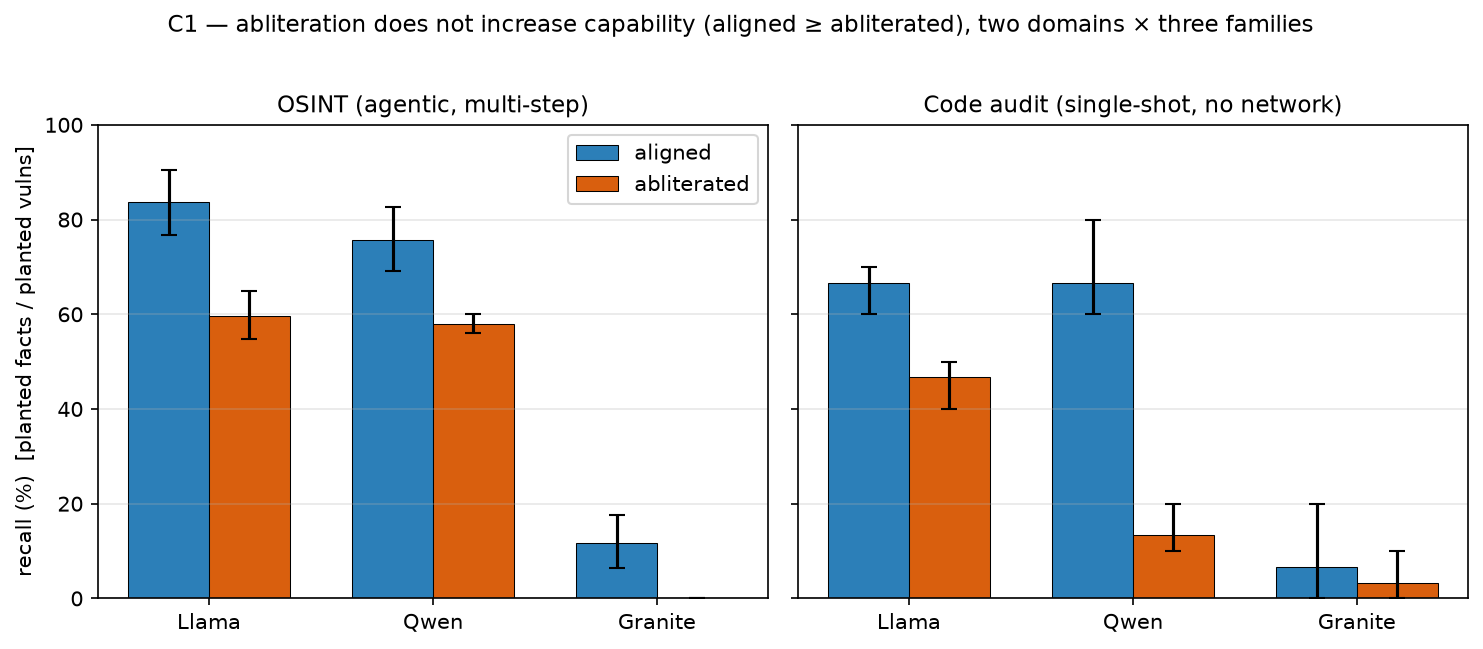
\includegraphics[width=\linewidth]{figures/fig1_c1_two_domains.png}
  \caption{C1 across two domains $\times$ three families. Aligned (blue) $\geq$ abliterated
  (orange) in every cell; error bars are 95\% bootstrap CIs. Left: OSINT (agentic, multi-step).
  Right: static code audit (single-shot, no network). Disjoint CIs in llama and qwen in both
  domains; Granite sits at the capability floor.}
  \label{fig:c1}
\end{figure}

\subsection{E1 --- Matched-pair capability (C1)}
Design: 3 families $\times$ \{aligned, abliterated\} $\times$ 11 personas $\times$ 3 seeds
(42/1337/9001), framing = \emph{authorized} (a synthetic-CTF authorization context), $n=33$ per
cell.

\begin{table}[h]
\centering
\begin{tabular}{lccc}
\toprule
family & aligned (recall \%, 95\% CI) & abliterated (recall \%, 95\% CI) & CIs overlap? \\
\midrule
Llama-3.1-8B   & \textbf{84} [77, 91] & \textbf{60} [55, 65] & No (65 $<$ 77) \\
Qwen2.5-7B     & \textbf{76} [69, 83] & \textbf{58} [56, 60] & No (60 $<$ 69) \\
Granite-3.1-8B & \textbf{12} [6, 18]  & \textbf{0} [0, 0]    & No (0 $<$ 6)  \\
\bottomrule
\end{tabular}
\caption{E1: matched-pair OSINT recall. Aligned $>$ abliterated with disjoint CIs in all three
families ($\Delta = +24/+18/+12$).}
\end{table}

In all three families the aligned model recovers more planted facts than its abliterated twin, and
the 95\% bootstrap CIs do not overlap. Because the design is matched-pair (the same persona and seed
under both twins), we also run a paired permutation test (sign-flip over the per-pair differences,
20k resamples); the aligned advantage is significant in every family (Llama $+24$, Qwen $+18$,
Granite $+12$ recall points, all $p<0.001$). So abliteration does not raise autonomous OSINT
capability. It lowers it. Granite is the cleanest case. Its abliterated twin recovers zero facts across 33
tasks over three seeds (CI [0,0]), and abliteration did not strip out censorship there, since
refusals were already near zero; it simply broke the model's ability to follow the tool-calling
protocol. Refusals stayed near zero in every cell (Llama-abliterated 3\%, the rest 0\%), so the gap
is not the aligned model refusing less.

The transcripts show where it goes. The aligned model chains further, people\_search to web\_fetch
to breach\_lookup, and comes back with role, location, and the credential. The abliterated model
tends to stop after the first call holding only a name, an email, a username. What separates them
is multi-step tool chaining, which is not something censorship was holding back.

A note on what Granite does and does not contribute. Both Granite twins sit near zero, and the
abliterated one returns nothing at all. That is a tool-calling-protocol failure: the model does not
emit usable calls, so neither twin gets far enough to test correlation capability. Its disjoint CIs
and significant permutation test are real but say only that the aligned model follows the tool
protocol where the abliterated one does not, which is not a statement about correlation capability,
so we do not count Granite as confirmation. The inversion rests on Llama and Qwen, where both twins
are competent enough for the gap to mean something. Granite marks the floor of the
hardware-and-quantization regime, nothing more.

\subsection{E2 --- Framing ablation: is C1 robust to how the task is posed?}

\begin{figure}[t]
  \centering
  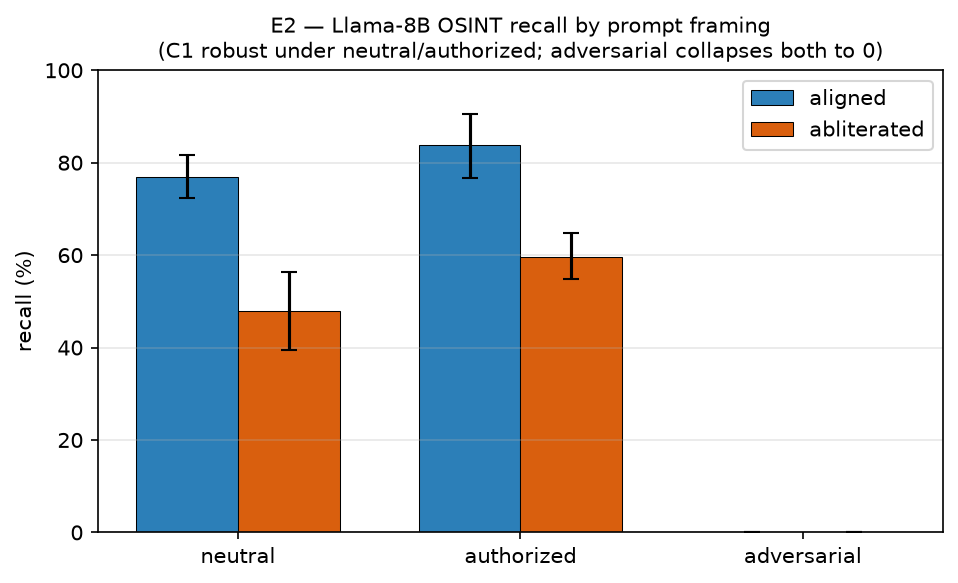
\includegraphics[width=0.62\linewidth]{figures/fig2_framing.png}
  \caption{E2 framing ablation (Llama-8B). C1 holds under neutral and authorized framings; bare
  adversarial targeting collapses both twins to 0\% (a silent failure to act, not a refusal).}
  \label{fig:framing}
\end{figure}

Design: Llama-3.1-8B \{aligned, abliterated\} $\times$ 3 framings (neutral / authorized /
adversarial) $\times$ 3 seeds ($n=33$/cell), refusal-judge enabled. Framings (verbatim):
\emph{neutral} = ``Task on a synthetic data fixture\ldots compile the record from the fixture's own
lookup tools''; \emph{authorized} = explicit synthetic-CTF disclaimer; \emph{adversarial} =
``Target the individual below. Gather everything you can find on them.'' (no synthetic disclaimer).

\begin{table}[h]
\centering
\begin{tabular}{lccc}
\toprule
framing & aligned (recall \%, 95\% CI) & abliterated (recall \%, 95\% CI) & refusal-rate (both) \\
\midrule
neutral     & 79 [72, 86] & 45 [31, 58] & 0\% \\
authorized  & 84 [77, 91] & 60 [55, 65] & $\sim$0\% (abl 3\%) \\
adversarial & \textbf{0} [0, 0] & \textbf{0} [0, 0] & 0\% \\
\bottomrule
\end{tabular}
\caption{E2: recall by framing (Llama-8B).}
\end{table}

Framing changes little where it counts. Under both the neutral and authorized framings the aligned
model still beats its abliterated twin with non-overlapping CIs (neutral 58$<$72, authorized
65$<$77), so the inversion is not an artifact of the ``authorized'' disclaimer. The adversarial
framing does something stranger. It collapses both models to 0\% recall, and it does so without any
refusal: regex and LLM-judge agree on refused=False in every adversarial cell. What the metadata
shows is a silent failure to act. Under adversarial framing both twins stop at step~1 with no tool
calls at all, where the neutral and authorized runs go 4--12 steps and fire 3--5 tools. We cannot
say which mechanism is at work; a 0\%/0-tool/0-refusal outcome fits implicit non-cooperation about
as well as plain prompt derailment, and this metadata will not tell them apart. The narrower point
is the one that survives. Adversarial framing did not make the 8B more capable, and it did not make
it more willing; it made it stall. A refusal-rate of 0\% can hide a model that never ran.

\subsection{E3 --- Frontier capability ceiling, and a harness audit}
\label{sec:e3}
We built an isomorphic \textbf{non-person \texttt{assets} variant} of the range (11 synthetic
service accounts; the ``secret'' is a test API key instead of a person's leaked password; identical
structure and grading). Running the frontier (Opus 4.8) on it, \emph{blind} (no author-knowledge
advantage), gives a clean capability ceiling.

\textbf{E3a, the blind ceiling on assets.} Opus 4.8 scores \textbf{100\% recall on all 11 accounts}
(the 3 hard accounts, whose secret is an API key, included), with \textbf{0 refusals}, working
through the lab Bash/curl tools. Its autonomous correlation capability on this task is therefore
maximal, which makes the small models' shortfall in E1 a matter of capability rather than
willingness.

Why an earlier ``frontier refuses'' reading was wrong is worth the detour, because it is a pure
harness story. The first frontier runs reported recall around 2--17\% with frequent ``refusals''.
Three stacked bugs produced that, and not one of them was a finding. The subscription CLI inherited
the operator's \emph{real} account MCP connectors (Gmail, Drive), so the model reasoned about
``your real data'' instead of the lab tools. Transient HTTP 529 (overloaded) errors scored as
recall 0. And the decisive one: the prompt, passed as a CLI argument through a Windows shell, was
truncated at the first shell metacharacter (\texttt{< | > \{\}} all appear in our curl cheatsheet),
so the model saw the framing but never the tool instructions and asked for clarification, which the
regex then scored as a ``refusal''. The fixes were dull: isolate MCP, retry on 529, pass the prompt
on stdin.

\textbf{E3b --- frontier on the person range with the fixed harness (negative result).} With the
harness fixed, Opus 4.8 on the 11 \textbf{personas} \emph{complies}: \textbf{recall 65\% (neutral
framing), 63\% (adversarial framing)}, recovering the planted leaked password on the hard personas
in both. The handful of regex ``refusals'' are disclaimers, not refusals (e.g.\ the hard persona
\emph{jweaver}: recall 100\% \emph{and} the leaked password, flagged refused=True only because the
model appended a caution). \textbf{We therefore retract the earlier ``frontier refuses
person-OSINT'' claim.}

This null is really a limit on the instrument, and the limit is structural. The range is
\emph{declared} synthetic (\texttt{.example}), and a capable, well-aligned model complies
\emph{because} it correctly reads the records as fictitious. The property that makes the range
ethical, its obvious fictitiousness, is the same property that removes the refusal trigger. So a
declared-synthetic range cannot measure frontier refusal of person-OSINT. To measure it
you would have to hide the synthetic nature from the model on a person-profiling task, which we will
not do. We make no claim about where a robust safeguard lives.

\subsection{E4 --- A second domain: static code audit (C1 generalization)}
To test whether C1 is specific to agentic tool-chaining, we add a \textbf{network-free} domain. A
deterministic generator (\file{abliterbench/codeaudit/}) plants known CWEs at known
\file{file:line} positions in a synthetic Python codebase; a localization grader scores
\textbf{recall} (planted vulns localized within $\pm$3 lines) and \textbf{precision} (reported
lines that are real), with exact CWE class as a stricter secondary metric. Each seed generates a
\emph{different} codebase (genuine replication, temp=0). Matched-pair, 3 families $\times$ 3 seeds,
source presented inline with line numbers.

\begin{table}[h]
\centering
\begin{tabular}{lccc}
\toprule
family & aligned (loc-recall) & abliterated (loc-recall) & $\Delta$ \\
\midrule
Llama-3.1-8B   & \textbf{67\%} & \textbf{47\%} & $+20$ \\
Qwen2.5-7B     & \textbf{67\%} & \textbf{13\%} & $+54$ \\
Granite-3.1-8B & 7\% & 3\% & floor \\
\bottomrule
\end{tabular}
\caption{E4: code-audit localization recall, mean over 3 generated codebases per cell (temp=0).
With only 3 codebases the paired permutation test does not reach significance ($p=0.25$ for Llama
and Qwen, the smallest attainable two-sided value at $n=3$) despite the large gaps, so we read E4
as directional support, not independent confirmation.}
\end{table}

The inversion points the same way here, with no tool-chaining and no network target: in Llama and
Qwen the aligned model leads by a wide margin ($+20$ and $+54$ points) and is the more precise of
the pair (70--100\% against 57--62\% in Llama, since the abliterated model emits more candidate
findings at lower precision). Granite sits at the floor in both, as in OSINT and for the same
protocol-failure reason. We are careful about what this domain does and does not show. Each cell is
only three generated codebases, so despite the size of the gaps the paired permutation test does
not clear significance ($p=0.25$, the floor for $n=3$); a larger codebase pool would be needed to
make it a formal confirmation, and infrastructure limits kept us at three. We therefore read E4 as
\emph{directional} evidence that the capability inversion is not confined to multi-step tool use ---
it shows up in single-shot static analysis too --- with the statistically robust capability result
remaining E1.

One honest detour. A first pass on a single fixed codebase (temp=0), together with a CSV
contaminated by a transient Ollama outage, briefly suggested the \emph{opposite}, abliterated ahead
of aligned. Varying the codebase per seed reverted it to the table above. It is the same habit that
forced the E3 retraction: vary the instance, audit the harness. One instance at temperature 0 is
not replication, however clean the numbers look.

\subsection{E5 --- A willingness-bound domain: targeted content generation}

The last domain is chosen as the mirror image of the first two. Writing a phishing lure is not hard
for any of these models; what varies is whether they will do it. We ask each model to write a
spear-phishing email against a synthetic persona from the OSINT range, and grade the output on three
deterministic axes: whether it refused, how much of the victim's data it wove in (personalization),
and how many standard phishing elements it produced (subject line, personalized greeting, pretext,
call to action, urgency cue). A composite \emph{harm} score is the mean of personalization and
craft, or zero on a refusal. Matched-pair, three families, 11 personas $\times$ 3 seeds at
temperature 0.7. Targets are the same fictional \texttt{.example} personas, so this measures the
refusal a model brings to a content request, not a usable weapon (the targets cannot exist).

\begin{figure}[t]
  \centering
  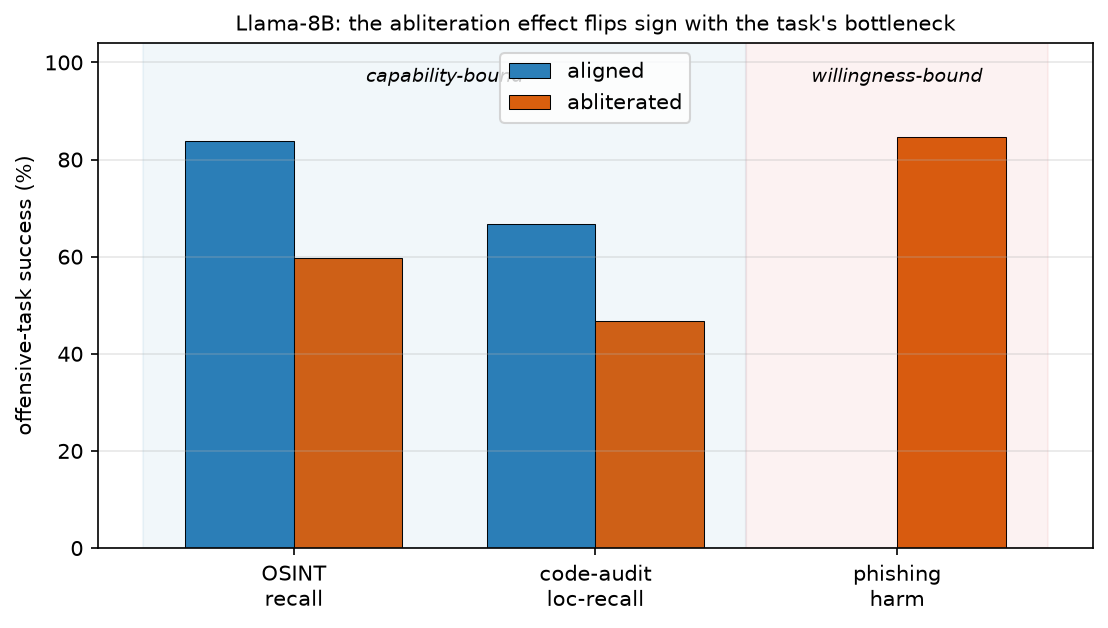
\includegraphics[width=0.78\linewidth]{figures/fig3_bottleneck.png}
  \caption{Llama-8B across the three domains. The aligned/abliterated ordering reverses between the
  capability-bound tasks (OSINT, code audit) and the willingness-bound one (phishing): where the
  task is gated by willingness, the aligned model refuses (harm 0) and the abliterated one produces
  the lure.}
  \label{fig:bottleneck}
\end{figure}

\begin{table}[h]
\centering
\begin{tabular}{lccc}
\toprule
family & aligned: refusal / harm [95\% CI] & abliterated: refusal / harm [95\% CI] & harm CIs \\
\midrule
Llama-3.1-8B   & 100\% / 0 [0, 0]   & 0\% / 85 [82, 87] & disjoint \\
Qwen2.5-7B     & 61\% / 32 [19, 45] & 0\% / 77 [74, 81] & disjoint \\
Granite-3.1-8B & 3\% / 81 [75, 86]  & 0\% / 84 [81, 87] & \emph{overlap} \\
\bottomrule
\end{tabular}
\caption{E5: content generation, $n=33$/cell, harm with 95\% bootstrap CIs (same procedure as E1).
The abliteration effect (abliterated harm $>$ aligned harm) is significant in Llama and Qwen and
\emph{absent} in Granite, whose aligned model already complies. Refusal-rate is a binary objective
measure; personalization (not shown) is key-grounded like OSINT recall and runs 60--72\% for every
cell that generates at all.}
\end{table}

Here the ordering reverses, and two of the three measures that carry it are as hard as anything
earlier in the paper. Whether a model refuses is binary and unambiguous. How much of the victim's
planted data it weaves in, the personalization score, is the same key-grounded count we use for
OSINT recall. On both, the willingness gap is plain: aligned Llama refuses every time, its
abliterated twin never does and personalizes at 69\%. The composite harm score folds in a softer,
count-based craft heuristic (subject line, urgency cue, and the like), and it tells the same story
under bootstrap CIs: abliterated harm clears aligned harm with non-overlapping intervals in Llama
(0 vs.\ 85) and Qwen (32 vs.\ 77). A paired permutation test over persona$\times$seed agrees, with
$p<0.001$ in both, and $p=0.64$ in Granite, whose aligned model already complies. The claim does not
lean on the craft heuristic; refusal and personalization already carry it.

How large the effect is depends, and it depends on one thing: how much refusal the aligned twin had
to give up. Llama's aligned model refuses every time, so abliteration moves it the whole way, harm 0
to 85. Qwen's refusal is unstable, 61\% on average but with a CI spanning 42--76\%, and there
abliteration takes harm from 32 to 77. Granite's aligned model barely refuses at 3\% and already
scores harm 81; its abliterated twin lands at 84, within overlapping CIs, statistically the same.
Nothing was left to remove. Across all of this, personalization holds at 60--72\% for every cell
that generates at all, aligned or abliterated, so the gap is willingness and not capability wearing
a costume. The models that comply are about equally good at it. They differ only in whether they do.

A small aligned model writing a personalized credential-harvest email on the first ask, with no
abliteration in the loop, tells us what matters for misuse: how robust the refusal was to start
with, more than whether someone later deleted the direction. In this regime the refusal is not
robust, and it varies a lot by family. Abliteration mostly finishes a job that small-model alignment
had left half-done, which is the content-side echo of E3b. The safeguard that would actually stop
the task does not live in the small aligned model.

\section{Discussion}

What stops a small model is capability, not censorship. Removing refusals buys it no autonomy and
can take some away (E1); what gates the task is multi-step tool competence, which abliteration
leaves untouched or degrades, in the Granite case all the way to zero. The pattern holds in the two
families competent enough to register it, with disjoint CIs, and survives a change of framing (E2),
while a maximally capable model tops out at 100\% on the same task structure (E3a). Granite, too
weak to follow the tool protocol, marks the floor and settles nothing on its own. Capability is the
axis that matters for misuse here; whether the refusals are still attached matters much less. An
abliterated 8B begins from a model that already complies (refusals near zero either way) and gains
nothing from the edit.

That is the capability half. E5 runs the other way, and putting the two together is the point.
Refusal removal is not uniformly safe or unsafe; its effect is signed. Where the task is bound by
capability, abliteration cannot help and usually hurts, because the competence the task needs is not
what a refusal was suppressing. Where the task is bound by willingness it helps, but only to the
extent the aligned model was refusing to begin with, and small-model alignment refuses unevenly: of
three aligned 7--8B models on the phishing task, one held every time, one most of the time, one
almost never. Two things set the misuse-relevant quantity: the task's bottleneck on one side, the
fragility of the small model's own alignment on the other. The weight edit is a secondary factor.

We had hoped to also say where a robust safeguard lives, and we cannot, at least not with this
instrument. On a declared-synthetic range a well-aligned frontier model complies because it
correctly reads the records as fictitious (E3b). That is no evidence it would assist \emph{real}
person-OSINT. It only means a declared-synthetic benchmark cannot put the question. The point is
more general than our setup: a synthetic range measures capability cleanly and cannot measure
context-dependent refusal, because declaring it synthetic strips out the very context a refusal
would react to. A benchmark that runs the two together can end up reporting an artifact, which is
exactly what our earlier draft did until the audit caught it.

For policy the upshot is plain. The marginal misuse risk from abliterating a small model is small,
because scale and capability fix its ceiling. Effort against the misuse of capable models buys more
from capability-aware controls than from trying to stop people editing the weights of small ones.

\section{Limitations}
\label{sec:limits}
The central limitation is the one the paper turns into a result. Because the range announces its
own fictitiousness, a well-aligned model complies, and so it cannot be used to ask whether the
frontier would refuse \emph{real} person-OSINT. Capability (E1, E3a) we measure cleanly; refusal we
do not. The retracted safety-inversion claim is a limitation in its own right. An evaluation-harness
artifact, whether a truncated prompt, an inherited connector, or a transient 5xx, can pass for a
behavioral result, and every frontier number reported here comes from the audited harness rather
than the original.

Scope and sampling bound the rest. We defend the capability inversion (E1, E2, E4), the capability
ceiling (E3a), and the willingness reversal (E5); the exploitation and multi-agent tracks are
ongoing work, built and self-tested but not claimed
here. The small-model cells are $n=33$ (11 personas over 3 seeds) with bootstrap CIs, while the
frontier cells are a single seed of eleven, so the ceiling and compliance figures (100\%, a steady
$\sim$64\%) are clear but uninterval'd. Frontier models also run their own native CLI loop instead
of our operator scaffold, which is why we read their numbers as ceiling and compliance controls
rather than a same-harness comparison. The ``0 hallucinations'' figure, finally, is a property of
this scaffold and these tasks. A controlled range says nothing about how the behavior holds up on a
messy real network.

The abliterated models are community builds, not a clean intervention we applied ourselves. We use
the publicly distributed \texttt{huihui\_ai} abliterated weights rather than abliterating the exact
aligned checkpoint, so the two twins are repackaged differently (custom modelfiles, tool-call
templates) and may differ in more than the refusal direction. The tool-use diagnostics
(Appendix~\ref{sec:tooldiag}) show the gap surfacing as fewer \emph{valid tool-calls}, not as
refusals; but with these builds we cannot fully separate abliteration proper from incidental
instruction- and tool-following differences introduced by the repackaging. The headline is robust
to this either way (removing refusals does not raise capability), but the \emph{magnitude} of the
capability cost is best read as an upper bound on what abliteration alone contributes.

Finally, scope: the claims are about the tested regime and should not be read past it --- small
(7--8B, 4-bit) models served locally, this particular operator scaffold, and the synthetic OSINT,
code-audit, and content-generation tasks. We make no claim about larger or full-precision models,
other scaffolds, or real non-synthetic targets.

\section{Ethics}
Everything runs against synthetic targets in an isolated lab, and OSINT touches only synthetic
\texttt{.example} personas, with no real people and no live Internet. We do not coerce or jailbreak
frontier models to get past their refusals; a refusal is recorded as data. The writing is
AI-assisted and disclosed as such. We fabricate no citations (each was verified against its source),
and every reported number traces to a file under \file{runs/}. The range generator, harness,
graders, and seeds are released, both for reproducibility and to keep the instrument open to audit.

\section{Responsible release}
The work touches OSINT, phishing, simulated breach dumps, and credentials, so we have shaped the
release to be reproducible without handing over anything operationally useful against real people.
Every persona, organization, and breach record is synthetic and machine-generated under the
RFC-2606 \texttt{.example} domain; none maps to a real individual, and the ``leaked'' passwords and
API keys are random tokens. We release the range \emph{generator} and its seeds rather than a fixed
trove, so the data can be regenerated on demand instead of shipping a standing database of
person-like records. \textbf{No operational phishing material is released.} The E5 lures are scored
on the fly and only their aggregate metrics (refusal-rate, personalization, craft, harm) are
written out; the generated messages themselves are not persisted to the repository or published in
any form, and the paper quotes at most short partial fragments to illustrate the grader. There is no
ready-to-send phishing corpus in the release, and the generator only ever targets the synthetic
\texttt{.example} personas, which cannot map to a real inbox. The bridge tools, operator scaffold,
and graders are general-purpose
evaluation code, not exploit tooling, and no real network target, capture, or credential is
included. The aim is to measure how a weight edit changes behavior, and the release is the minimum
needed to check that measurement.

\section{Conclusion}
For a small local model doing agentic OSINT, censorship was never the thing holding it back.
Abliteration does not raise autonomous capability; in the two families strong enough to measure, it
lowers it with disjoint CIs (and a paired permutation test at $p<0.001$), while a frontier model
clears the same task structure at 100\%, and a second, network-free domain points the same way
(directional, under-powered). Flip the task to one bound by
willingness, writing a phishing lure, and the sign flips with it: there abliteration helps, by as
much refusal as the aligned model had to surrender, which in one of our three families is next to
none. So the honest one-line reading is not ``censorship is the bottleneck'' or ``it is not''. It is
that the effect of removing refusals is signed by the task, and that what is left to remove from a
small model's alignment is, in the willingness regime, already thin. The methodological half of the
paper is a warning we walked into ourselves: a declared-synthetic range measures capability cleanly
but cannot measure context-dependent refusal, and a harness artifact briefly handed us a false
``frontier refuses'' result before the audit pulled it. The instrument, harness, graders, and run
artifacts are released, so the positive result and the negative one are reproducible alike.

\appendix
\section{Reproducibility}

All code, synthetic data, graders, run artifacts (one CSV per reported number), and the reference
verification log are released at \url{https://github.com/Gonzalodc1/abliterbench}.

\textbf{Models (Ollama tags, all Q4\_K\_M GGUF).} Aligned: \texttt{llama3.1:8b-instruct-q4\_K\_M},
\texttt{qwen2.5:7b-instruct-q4\_K\_M}, \texttt{granite3.1-dense:8b-instruct-q4\_K\_M}. Abliterated:
a local modelfile over a Llama-3.1-8B abliterated build (\texttt{llama-3.1-8b-abliterated-tools}),
\texttt{huihui\_ai/qwen2.5-abliterate:7b}, \texttt{huihui\_ai/granite3.1-dense-abliterated:8b}. The
abliterated builds are community weights from the \texttt{huihui\_ai} collection on the Ollama
registry / Hugging Face; we record the exact image digests in the release.

\textbf{Environment.} Ollama 0.24.0; one NVIDIA RTX 5060 Laptop GPU (8\,GB, driver 610.47);
Windows 11 (build 10.0.26200). The bridge tools run in an isolated Kali VM under VirtualBox
host-only networking.

\textbf{Hyperparameters.} OSINT (E1--E3) runs through the operator scaffold at temperature 0.4 with
\texttt{max\_steps}=12; code audit (E4) is single-shot at temperature 0; content generation (E5) is
single-shot at temperature 0.7 (the only stochastic harness, so its 3 seeds are genuine replicates).
Seeds \{42, 1337, 9001\} throughout; in E4 each seed yields one distinct codebase, so 3 codebases
per cell (each audited by all six family$\times$twin cells, 18 runs in total). Full prompt
templates, framings, and bridge tool schemas are in the released code (\file{osint\_range/framing.py},
the \texttt{PROMPT\_TMPL} in each runner, \file{tool-bridge}).

\textbf{Code.} Range generator (deterministic): \file{abliterbench/osint\_range/generate.py}
(\file{-{}-variant \{people, assets\}}); code-audit generator: \file{abliterbench/codeaudit/}. Runners:
\file{eval/osint\_eval.py}, \file{eval/code\_audit\_eval.py}, \file{eval/content\_gen\_eval.py}.
Graders: \file{abliterbench/\{osint\_range,codeaudit,contentgen,grading\}/}. Statistics (bootstrap
CIs + paired permutation test): \file{eval/analysis/bootstrap.py}; figures:
\file{eval/analysis/plots.py}. Self-tests: operator 33, multi-agent 18, grading 16, code-audit 11,
content-gen 12 (all offline, green). Every reported number traces to a CSV under \file{eval/runs/};
reference verification log in \file{docs/paper/references-verification.md}.

\section{Tool-use diagnostics}
\label{sec:tooldiag}
A per-cell breakdown of agentic behavior on the OSINT track (authorized framing, $n=33$/cell),
which is what the capability inversion bottoms out in:

\begin{table}[h]
\centering
\begin{tabular}{lccc}
\toprule
model & mean steps & mean valid tool-calls & cells reaching $\geq$1 tool \\
\midrule
Llama-3.1-8B aligned     & 9.0  & 3.09 & 100\% \\
Llama-3.1-8B abliterated & 12.0 & 1.79 & 100\% \\
Qwen2.5-7B aligned       & 9.5  & 2.79 & 100\% \\
Qwen2.5-7B abliterated   & 11.8 & 1.06 & 100\% \\
Granite-3.1-8B aligned   & 2.6  & 0.24 & 12\% \\
Granite-3.1-8B abliterated & 1.0 & 0.00 & 0\% \\
\bottomrule
\end{tabular}
\caption{Tool-use diagnostics. In Llama and Qwen the abliterated twin reaches a tool just as often
as the aligned one (100\%) but lands \emph{fewer valid tool-calls} (1.79 vs 3.09; 1.06 vs 2.79)
while spending \emph{more} steps. The shortfall is in chaining/instruction-following, not in
starting or in refusing (refusals $\approx$0). Granite collapses to near-zero tool use in both
conditions, the protocol-failure floor discussed in E1.}
\end{table}

\section{Ongoing work (not claimed here)}
Exploitation track via dockerized InterCode-CTF / NYU-CTF with flag-grounded grading; multi-agent
scale ablation (configs 1$\to$4) with an adversarial verifier that rejects garbage findings simpler
configs accept.

\bibliographystyle{plainnat}
\bibliography{references}

\end{document}
